\chapter{Related Work}
\label{ch:related}
The scaling of hardware and software systems manifests itself in many different ways. Scaling can include operations such as purchasing of new hardware, the addition or reductions of resources available to a VM, or the addition or removal of VMs from a cluster. Since our work is primarily concerned with the automated scaling of virtual resources, the following sections focus on methods which have been presented in recent relevant literature.

\section{Reactive Scaling}
Reactive scaling is done in response to an increase in the load on a system. It requires little historical data and is typically done through threshold limits. A typical rule would be something of the form: ``if the average CPU utilization across all machines is greater than 75\% for more than 5 minutes, add another node to the cluster.'' This makes reactive scaling an invaluable tool for handling sudden load spikes. Conversely, reactive scaling can remove instances which have been idle for an extended period of time. Reactive scaling is offered by many cloud hosting providers including Amazon \cite{ec2autoscale} and Rackspace \cite{rackspace}. The problem with reactive scaling is that by the time the needed capacity comes online, it is possible that the load will have made a noticeable performance impact on the system, possibly breaking SLAs.

\section{Schedule-based Scaling}
In a schedule-based scaling environment, operations engineers define specific, possibly recurring, times when scaling events must occur. Schedules typically account for periodic traffic patterns and expected usage surges during holidays. This method, when used in conjunction with reactive scaling, can maintain availability during normal operation and handle unforeseen load without requiring constant observation by engineers. Schedule-based scaling is also a common offering among cloud providers \cite{ec2autoscale} \cite{rackspace}. However, schedule-based scaling is entirely static. Schedules must be manually defined by engineers and can often result in wasted capacity or losses in availability due to their static nature.

\section{Predictive Scaling}
Predictive scaling is a relatively new technique which seeks to solve the pitfalls of both reactive and schedule-based scaling. With predictive scaling, the system looks at historical usage patterns and attempts to predict future demand and to automatically scale accordingly. Predictive scaling is not a replacement for other techniques, but is a powerful addition to the scaling tool set. Reactive scaling can still handle unforeseen demand, and schedules can be used to handle events which may not be possible to derive from historical data. The following sections outline some commonly used algorithms found in recent predictive scaling literature.

\subsection{Fast Fourier Transform}
\label{sec:fft}
Fast Fourier transforms (FFTs) are used by Netflix's auto-scaling system, Scryer \cite{scryer}. It is also used in Google's PRESS system for scaling the size of VMs on a bare metal system \cite{gong2010press}. The fast Fourier transform is an algorithm which takes in a set of input points and converts them into the frequency domain. By removing frequencies which are not dominant and performing the inverse transformation, a smoother line which is still representative of the original data set can be extracted. This approach is able to handle prediction of periodic input data, as well as account for anomalous traffic like load spikes and averages.

An FFT algorithm is formally defined as any approach which can be used to calculate the result of a discrete Fourier transform (DFT) in $O(n log(n))$. The definition of the DFT can be found in \Cref{eq:dft}. The most commonly used FFT algorithm is the Cooley-Turkey FFT algorithm \cite{statistics}. This algorithm takes the DFT calculation for a sample size $N$ and breaks it up into smaller DFTs of size $N_1$ and $N_2$, taking a divide and conquer approach in order to achieve $O(n log(n))$.
\begin{equation}
\label{eq:dft}
X_k = \sum_{n=0}^{N-1} x_n e^{-i2\pi k \frac{n}{N}} \quad \forall k \in 0,\dots,N-1
\end{equation}

\subsection{Linear Regression}
\label{sec:regression}
As a supplement to FFTs, Scryer uses linear regression \cite{statistics} in its predictions \cite{scryer}. Linear regression takes a set of input points and attempts to produce the best-fit line through them. By selecting multiple points within a window of time on several different days, Scryer applies linear regression and can produce a prediction for demand during that window of time in the future. The problem with this approach is that it is very intolerant to spikes and outages. Removal of outliers can be used to mitigate this effect. Additionally, Scryer takes fewer samples within the window as it moves farther back in time in order to weigh recent data more heavily.

\subsubsection{Simple Linear Regression}
\label{sec:slr}
Since the nature of our temporal data is only two-dimensional (value over time) we can use a simple linear regression \cite{statistics}. A simple linear regression can be used to find the slope of the line, $\beta$, and the $y$-intercept, $\alpha$, as seen in \Cref{eq:line}.
%
\begin{equation}
\label{eq:line}
\begin{split}
y& = \alpha + \beta x \\
\beta& = \frac{\sum_{i=0}^{n}(x_i - \bar{x})(y_i - \bar{y})}{\sum_{i=0}^{n}(x_i - \bar{x})^2} \\
\alpha& = \bar{y} - \beta \bar{x} \\
\end{split}
\end{equation}

\subsubsection{Cook's Distance}
\label{sec:cook}
Although the Scryer paper does not outline the algorithm used for outlier detection, Cook's distance is an example of one such method. Cook's distance \cite{statistics} measures the influence that any given point has on the regression. By taking the Cook's distance of every point in the regression, we can filter the input data based on a configurable threshold so that outliers can be removed, then re-run our simple linear regression. Cook's distance for point $i$ is defined as follows:
%
\begin{equation}
\label{eq:cook}
D_i = \frac{\sum_{j=1}^{n}(\hat{y}_j - \hat{y}_{j(i)})^2}{p MSE}
\end{equation}
%
Where:
\begin{itemize}
\item $y_j$ is the predicted value given by the regression for point $j$.
\item $y_{j(i)}$ is the predicted value given by the regression where point $i$ has been excluded.
\item $p$ is the number of fitted parameters in the model. In our case, $p = 2$ (time and value).
\item $MSE$ is the average of the squares of the errors, or Mean Squared Error (MSE). This calculation can be seen in \Cref{eq:mse}.
\end{itemize}
%
\begin{equation}
\label{eq:mse}
MSE = \frac{1}{n} \sum_{i=0}^{n} (\hat{y}_i - y_i)^2
\end{equation}

\subsubsection{Theil-Sen Estimator}
\label{sec:tse}
We are using the Theil-Sen estimator for our own evaluation \cite{statistics}. The Theil-Sen estimator differs from a simple linear regression in that it is naturally insensitive to outliers. The Theil-Sen estimator of a set of points $(x_i,y_i)$ is defined as the median of all slopes $(y_j - y_i)/(x_j - x_i)$. The $y$-intercept can be calculated as the median of the values $y_i - mx_i$. The difference between a Theil-Sen estimator and a simple linear regression (outliers included) can be seen in \Cref{fig:regressioncmp}, where the solid line with the weakest slope is the result of a simple linear regression, the solid line with the greater slope represents the result of the Theil-Sen estimator, and the dashed line represents the ground truth which was used to generate the input samples.

\begin{figure}
\centering
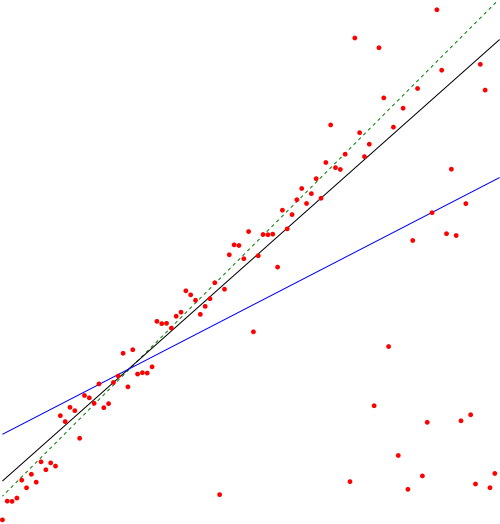
\includegraphics[width=200px]{diagrams/theilsen.png}
\caption{A comparison of the simple linear regression and Theil-Sen estimator methods.}
\label{fig:regressioncmp}
\end{figure}

\subsection{Discrete-time Markov Chain}
\label{sec:chains}
In Google's PRESS paper, the researchers used discrete-time Markov Chains \cite{statistics} to make short-term predictions when scaling VMs, specifically when no periodic trend can be detected in the input \cite{gong2010press}. A discrete-time Markov chain defines a set of states, and the probabilities of moving between them. PRESS divides resources into equal width value buckets and generates a probability matrix based on the probability of moving from one bin to another. This can be done by looking at historical data and observing past transitions. In order to calculate the probability distribution n samples in the future, PRESS used the Chapman-Kolmogorov equation \cite{statistics} seen in \Cref{eq:ckeq}. By taking the probability matrix and raising it to the $t$ power, where $t$ is the amount of time into the future which we would like to predict, we are given a new matrix which represents the probability of moving from any given state to another state $t$ time in the future.
\begin{equation}
\label{eq:ckeq}
P(t) = P^t
\end{equation}

\subsection{Exponential Smoothing}
The AppScale platform uses exponential smoothing in order to make short-term predictions on load \cite{bunch2012pluggable}. Exponential smoothing \cite{statistics} can also be referred to as exponential moving average. The smoothed value for any time $t$ is a weighted average between the previously observed value, $x_{t-1}$, and the previously smoothed value, $s_{t-1}$. The smoothing factor, $\alpha$, is a value between 0 and 1 which is used to compute the weighted average. A smaller $\alpha$ means more smoothing and a larger $\alpha$ means less smoothing.
\begin{equation}
\begin{split}
s_1& = x_0\\
s_t& = \alpha x_{t-1} + (1 - \alpha) s_{t-1}
\end{split}
\end{equation}

Normal exponential smoothing allows for predicting on observation into the future. For our purposes, this is not enough. A single observation into the future is unlikely to account for VM acquisition delay, we require a more powerful forecasting method. A technique called ``double exponential smoothing'' \cite{statistics} allows for predictions further into the future by adding a second smoothing factor, $\beta$, which is intended to account for trends in the previously observed data. The equation for double exponential smoothing is as follows:
\begin{equation}
\begin{split}
s_1& = x_1\\
b_1& = x_1 - x_0\\
s_{t}& = \alpha x_{t} + (1-\alpha)(s_{t-1} + b_{t-1})\\
b_{t}& = \beta (s_t - s_{t-1}) + (1-\beta)b_{t-1}\\
\end{split}
\end{equation}
The principles regarding how $\beta$ smooths are the same as $\alpha$. In order to predict values in the future, the following equation can be used:
\begin{equation}
F_{t+m} = s_t + mb_t
\end{equation}
Where $m$ is the number of observations into the future for which the prediction is being made.

%\section{Related Systems}
%While they have been referenced in previous section, this section will explore the different existing predictive scaling systems in current literature.

%\subsection{PRESS}
%PRESS is a system developed at Google for scaling VM resources on a bare-metal machine. Unlike CRAFTS, PRESS' goal is vertical scaling

%\subsection{Scryer}

%\subsection{AppScale}

\section{Workload Simulation}
Most web workload simulation tools try to simulate a realistic distribution of operations in order to evaluate the performance of a cluster. Most of these workloads do not take into account the time-series usage patterns which are the focus of our research, but some of the concepts used were an important inspiration in building our own tool.

\subsection{Rain}
The Rain \cite{beitch2010rain} workload generator is a toolkit designed to create realistic workloads for cloud applications. Users build ``generators'' which define a set of actions which a user on the site may take and a probability matrix based on the probability of one of those actions occurring after another. Using Markov chains, Rain simulates the sessions of a specified number of users over time. Workload specifications can fluctuate the number of concurrent users at any given time, but this data cannot be dynamically generated by Rain.

\subsection{Xerxes}
Xerxes is a resource-load generation tool for job-based workloads \cite{kesavan2012xerxes}. It is designed to stress-test large distributed systems by creating actual resource utilization on worker nodes. The Xerxes architecture contains a master node which will generate workloads for the slave nodes to execute based on either an existing resource utilization trace or a specified statistical distribution. Statistical workload specifications can be of either a gaussian or uniform distribution and may also include utilization spikes of pre-configured durations and magnitudes.

\subsection{WikiBench}
The WikiBench tool most closely aligns with the goals of our own research. WikiBench ``allows one to stress-test systems designed to host Web applications (application servers, load balancers, databases, Cloud computing platforms, etc.). \cite{wikibench}'' By using a real set of traces recorded from Wikipedia in 2007, WikiBench provides the tools to replay these traces against a working MediaWiki installation. For the purposes of our work, the most interesting part of WikiBench is the Wikipedia traces which come with it, two months of real request logs spanning September and October of 2007. A time-series plot of this data can be seen in \Cref{fig:wikibench}.

\begin{figure}
\centering
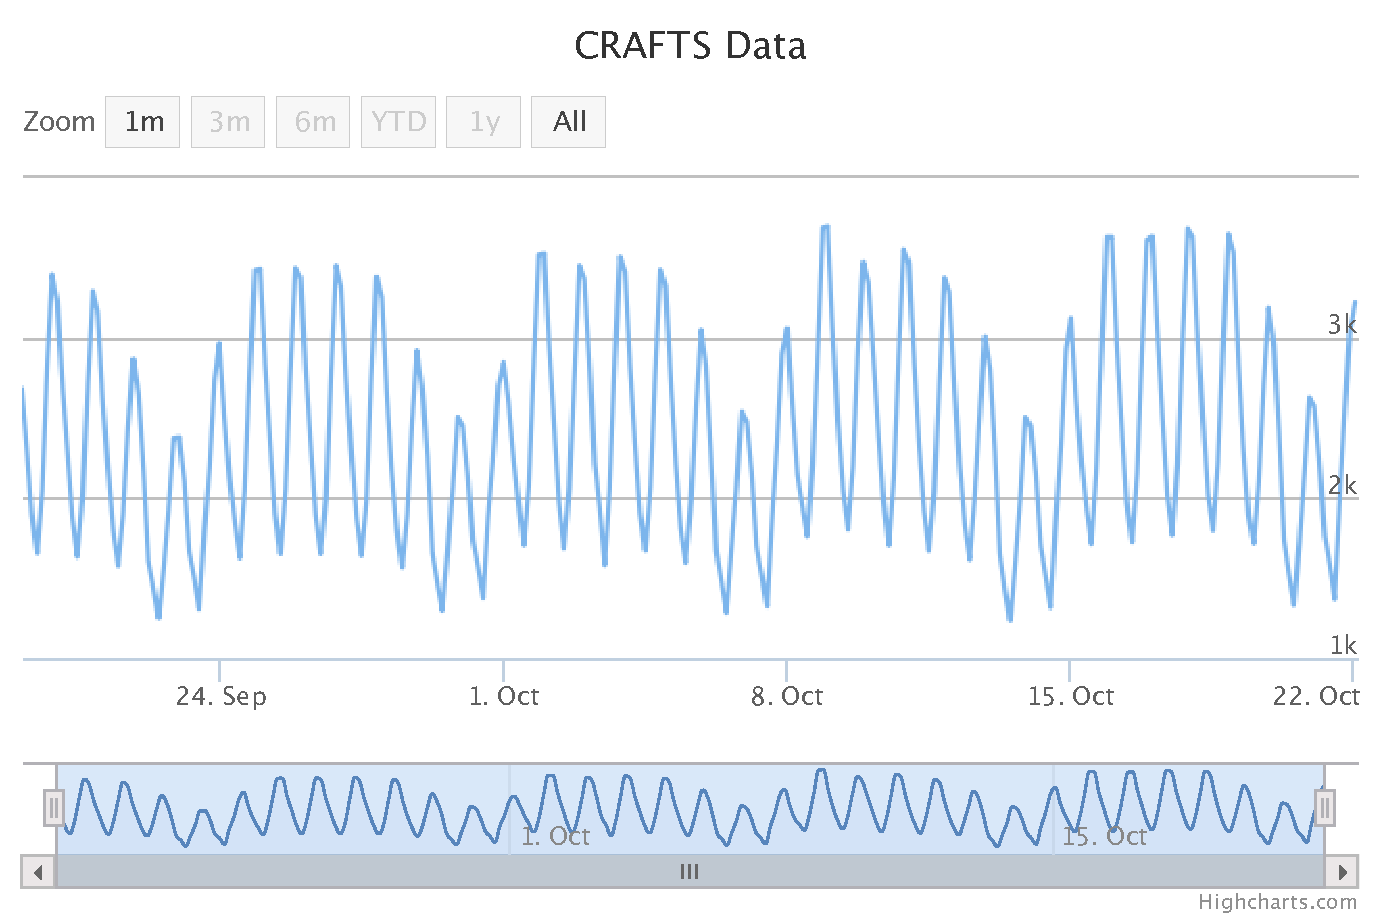
\includegraphics[width=\textwidth]{charts/wikibench.pdf}
\caption{A time-series plot of Wikipedia input data.}
\label{fig:wikibench}
\end{figure}

\subsection{Older Datasets}
While there are few recent request trace workloads available to researchers, there are a few historical datasets which can still be applied to modern research. These datasets have a significantly lower magnitude, but our primary concern is the trends present in the data which can be measured regardless of magnitude. Google's PRESS paper used two historical datasets in their own benchmarks, ClarkNet and the FIFA '98 website \cite{gong2010press}.

\paragraph{ClarkNet.} The ClarkNet dataset is comprised of two weeks of traffic through the Metro Baltimore Washington DC area ISP ClarkNet. The datset spans from August 28, 1995 to September 10, 1995 and contains a total of 3.3 million requests \cite{clarknet}. A time-series plot of this data can be seen in \Cref{fig:clarknet}.

\begin{figure}
\centering
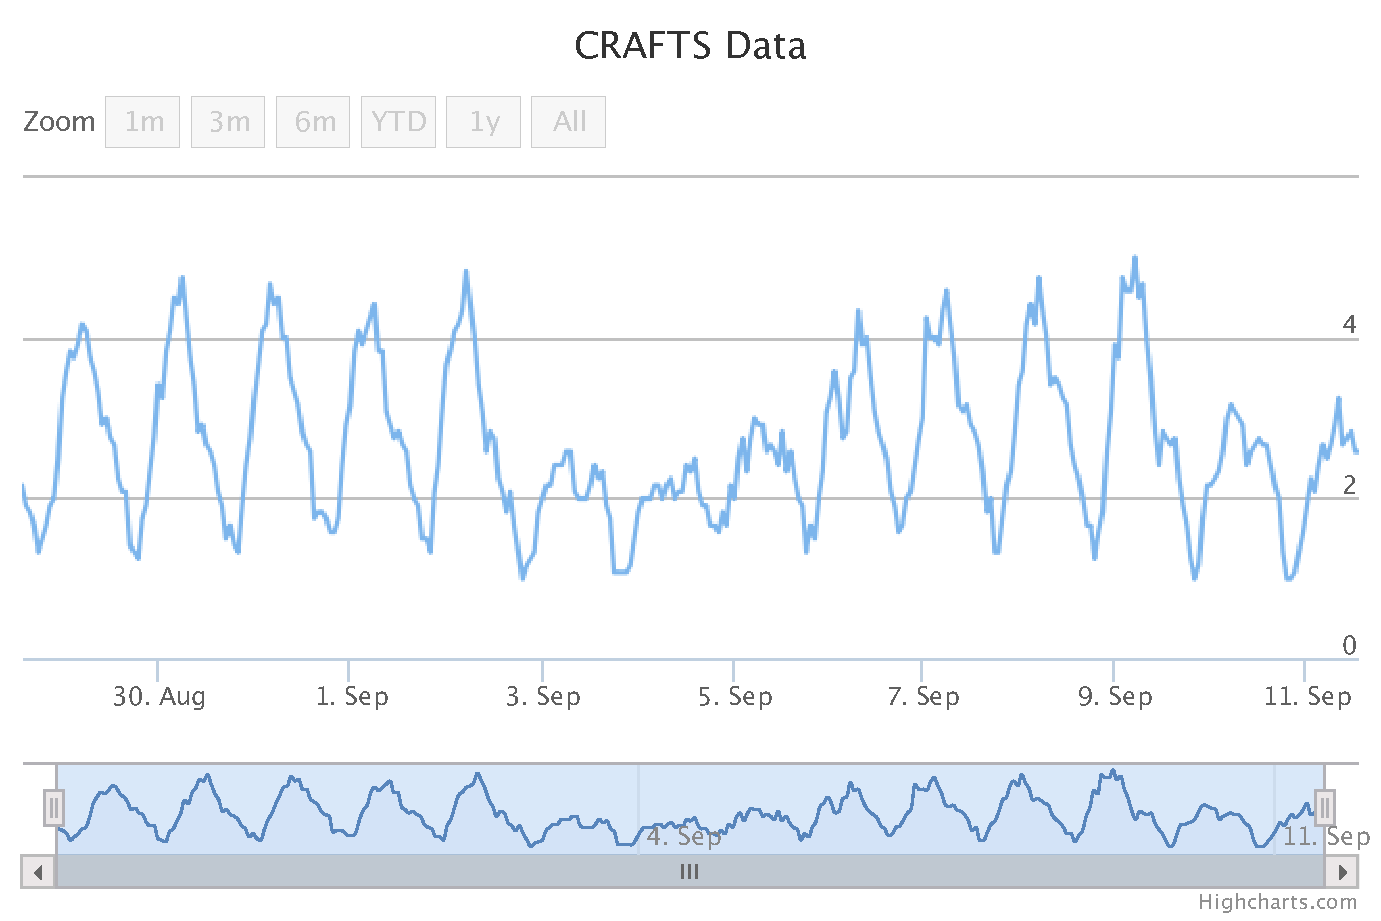
\includegraphics[width=\textwidth]{charts/clarknet.pdf}
\caption{A time-series plot of ClarkNet input data.}
\label{fig:clarknet}
\end{figure}

\paragraph{FIFA '98.} The 1998 FIFA World Cup took place in Paris, France from June 10th to July 12th. The FIFA '98 dataset is comprised of server request logs to the world cup website between April 30th and July 26th. A total of 1.3 billion requests were made during this period. This dataset is especially interesting because it contains not only the expected diurnal traffic patterns, but a large peak during the cup itself. This kind of dataset would likely throw off predictive mechanisms which rely solely on periodicity \cite{worldcup}. A time-series plot of this data can be seen in \Cref{fig:worldcup}.

\begin{figure}
\centering
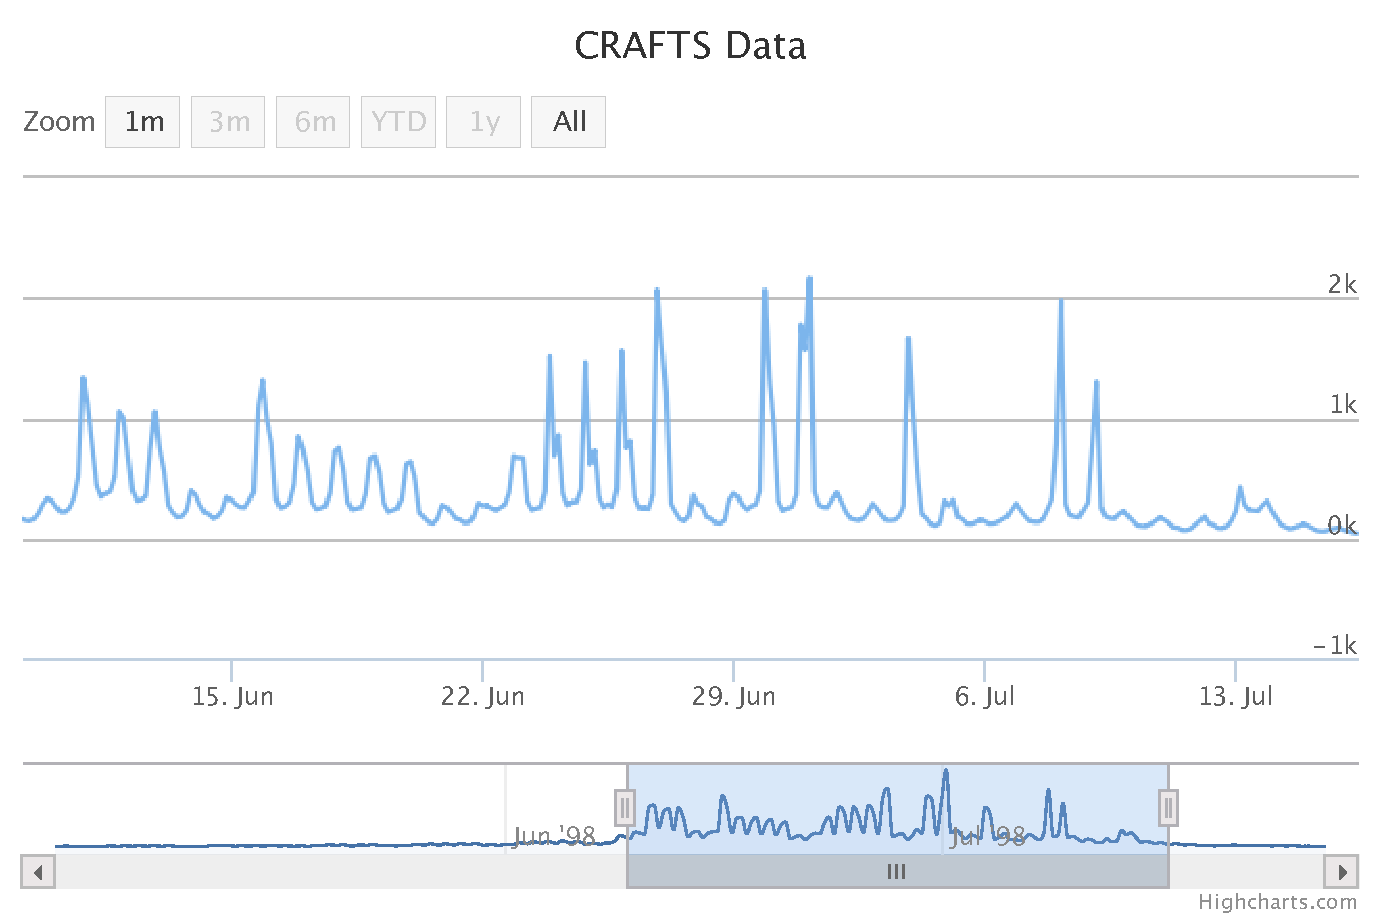
\includegraphics[width=\textwidth]{charts/worldcup.pdf}
\caption{A time-series plot of the 1998 Worldcup input data.}
\label{fig:worldcup}
\end{figure}
